\documentclass{standalone}
\usepackage{tikz}
\usetikzlibrary{patterns, positioning}

\begin{document}
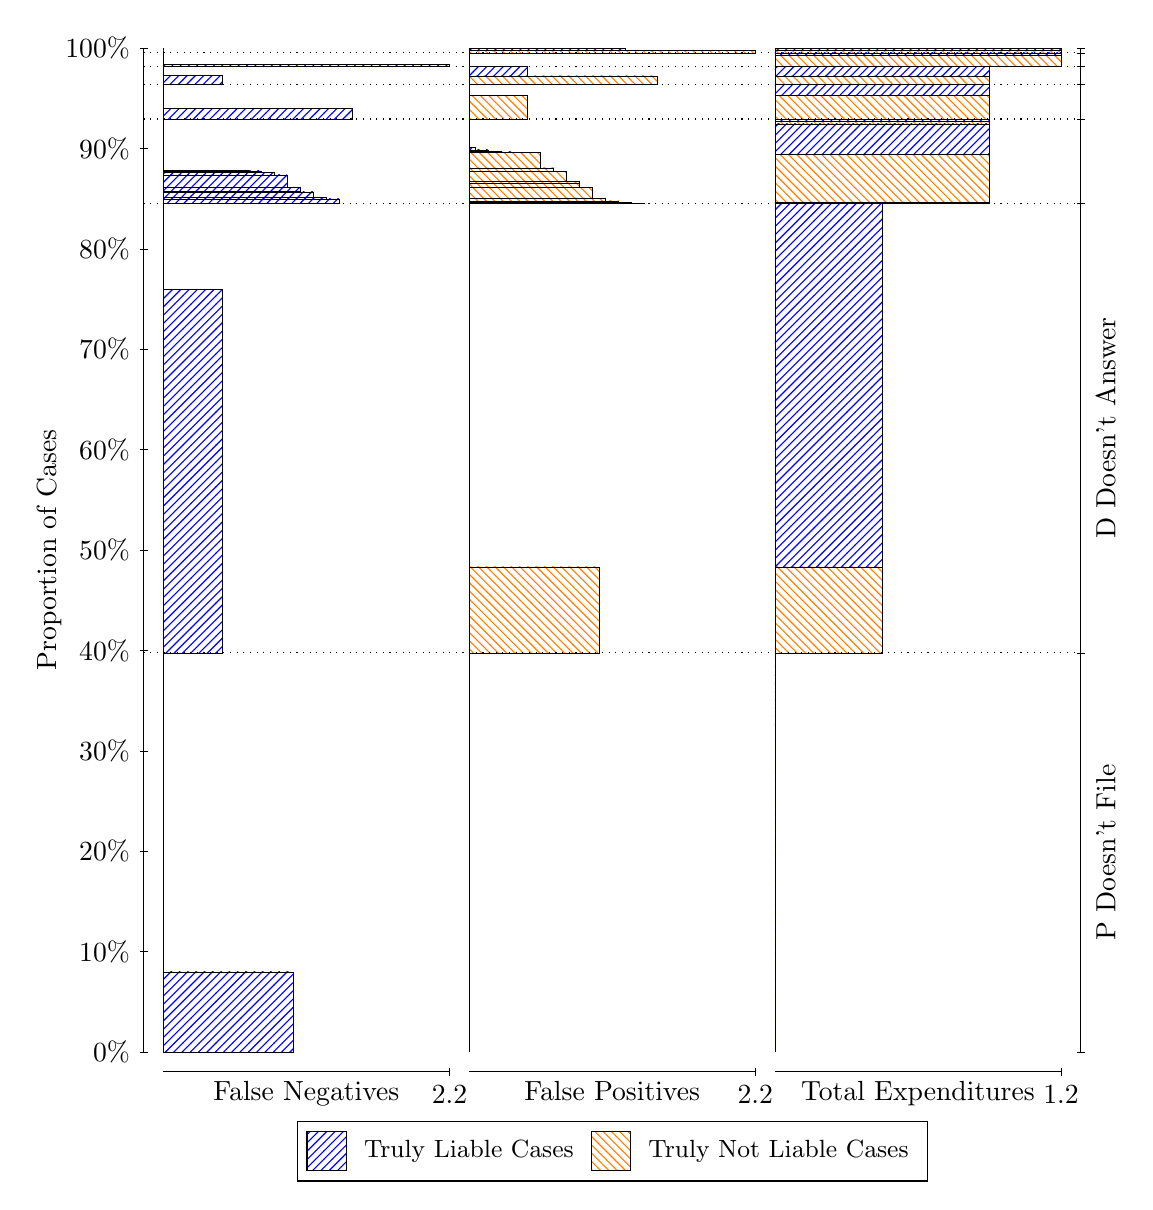
\begin{tikzpicture}
\draw[black, very thin] (1.5,1.75) -- (1.5,14.5);
\node[rotate=90, anchor=center] at (0.3, 8.125) {Proportion of Cases};
\draw[black, very thin] (1.45,1.75) -- (1.55,1.75);
\node[anchor=east] at (1.45, 1.75) {0\%};
\draw[black, very thin] (1.45,3.025) -- (1.55,3.025);
\node[anchor=east] at (1.45, 3.025) {10\%};
\draw[black, very thin] (1.45,4.3) -- (1.55,4.3);
\node[anchor=east] at (1.45, 4.3) {20\%};
\draw[black, very thin] (1.45,5.575) -- (1.55,5.575);
\node[anchor=east] at (1.45, 5.575) {30\%};
\draw[black, very thin] (1.45,6.85) -- (1.55,6.85);
\node[anchor=east] at (1.45, 6.85) {40\%};
\draw[black, very thin] (1.45,8.125) -- (1.55,8.125);
\node[anchor=east] at (1.45, 8.125) {50\%};
\draw[black, very thin] (1.45,9.4) -- (1.55,9.4);
\node[anchor=east] at (1.45, 9.4) {60\%};
\draw[black, very thin] (1.45,10.675) -- (1.55,10.675);
\node[anchor=east] at (1.45, 10.675) {70\%};
\draw[black, very thin] (1.45,11.95) -- (1.55,11.95);
\node[anchor=east] at (1.45, 11.95) {80\%};
\draw[black, very thin] (1.45,13.225) -- (1.55,13.225);
\node[anchor=east] at (1.45, 13.225) {90\%};
\draw[black, very thin] (1.45,14.5) -- (1.55,14.5);
\node[anchor=east] at (1.45, 14.5) {100\%};

\draw[black, very thin] (13.4,1.75) -- (13.4,14.5);
\draw[black, very thin] (13.35,1.75) -- (13.45,1.75);
\node[anchor=west] at (13.35, 1.75) {};
\draw[black, very thin] (13.35,6.8187) -- (13.45,6.8187);
\node[anchor=west] at (13.35, 6.8187) {};
\draw[black, very thin] (13.35,12.528) -- (13.45,12.528);
\node[anchor=west] at (13.35, 12.528) {};
\draw[black, very thin] (13.35,13.598) -- (13.45,13.598);
\node[anchor=west] at (13.35, 13.598) {};
\draw[black, very thin] (13.35,14.038) -- (13.45,14.038);
\node[anchor=west] at (13.35, 14.038) {};
\draw[black, very thin] (13.35,14.265) -- (13.45,14.265);
\node[anchor=west] at (13.35, 14.265) {};
\draw[black, very thin] (13.35,14.438) -- (13.45,14.438);
\node[anchor=west] at (13.35, 14.438) {};
\draw[black, very thin] (13.35,14.5) -- (13.45,14.5);
\node[anchor=west] at (13.35, 14.5) {};

\draw[black, very thin, pattern color=blue, pattern=north east lines] (1.75,1.75) rectangle (3.4015,2.768);
\draw[black, very thin, pattern color=orange, pattern=north west lines] (1.75,2.768) rectangle (1.75,6.8187);
\draw[black, very thin, pattern color=blue, pattern=north east lines] (1.75,6.8187) rectangle (2.4932,11.437);
\draw[black, very thin, pattern color=orange, pattern=north west lines] (1.75,11.437) rectangle (1.75,12.528);
\draw[black, very thin, pattern color=blue, pattern=north east lines] (1.75,12.528) rectangle (3.9795,12.583);
\draw[black, very thin, pattern color=blue, pattern=north east lines] (1.75,12.583) rectangle (3.8144,12.599);
\draw[black, very thin, pattern color=blue, pattern=north east lines] (1.75,12.599) rectangle (3.6492,12.672);
\draw[black, very thin, pattern color=blue, pattern=north east lines] (1.75,12.672) rectangle (3.4841,12.683);
\draw[black, very thin, pattern color=blue, pattern=north east lines] (1.75,12.683) rectangle (3.4841,12.728);
\draw[black, very thin, pattern color=blue, pattern=north east lines] (1.75,12.728) rectangle (3.3189,12.889);
\draw[black, very thin, pattern color=blue, pattern=north east lines] (1.75,12.889) rectangle (3.1538,12.919);
\draw[black, very thin, pattern color=blue, pattern=north east lines] (1.75,12.919) rectangle (2.9886,12.94);
\draw[black, very thin, pattern color=blue, pattern=north east lines] (1.75,12.94) rectangle (2.8235,12.945);
\draw[black, very thin, pattern color=blue, pattern=north east lines] (1.75,12.945) rectangle (2.6583,12.948);
\draw[black, very thin, pattern color=orange, pattern=north west lines] (1.75,12.948) rectangle (1.75,13.598);
\draw[black, very thin, pattern color=blue, pattern=north east lines] (1.75,13.598) rectangle (4.1447,13.737);
\draw[black, very thin, pattern color=orange, pattern=north west lines] (1.75,13.737) rectangle (1.75,14.038);
\draw[black, very thin, pattern color=blue, pattern=north east lines] (1.75,14.038) rectangle (2.4932,14.156);
\draw[black, very thin, pattern color=orange, pattern=north west lines] (1.75,14.156) rectangle (1.75,14.265);
\draw[black, very thin, pattern color=blue, pattern=north east lines] (1.75,14.265) rectangle (5.3833,14.293);
\draw[black, very thin, pattern color=orange, pattern=north west lines] (1.75,14.293) rectangle (1.75,14.438);
\draw[black, very thin, pattern color=orange, pattern=north west lines] (1.75,14.438) rectangle (1.75,14.466);
\draw[black, very thin, pattern color=blue, pattern=north east lines] (1.75,14.466) rectangle (1.75,14.5);
\draw[black, very thin, pattern color=orange, pattern=north west lines] (5.6333,1.75) rectangle (5.6333,5.8008);
\draw[black, very thin, pattern color=blue, pattern=north east lines] (5.6333,5.8008) rectangle (5.6333,6.8187);
\draw[black, very thin, pattern color=orange, pattern=north west lines] (5.6333,6.8187) rectangle (7.2848,7.91);
\draw[black, very thin, pattern color=blue, pattern=north east lines] (5.6333,7.91) rectangle (5.6333,12.528);
\draw[black, very thin, pattern color=orange, pattern=north west lines] (5.6333,12.528) rectangle (7.8629,12.531);
\draw[black, very thin, pattern color=orange, pattern=north west lines] (5.6333,12.531) rectangle (7.6977,12.536);
\draw[black, very thin, pattern color=orange, pattern=north west lines] (5.6333,12.536) rectangle (7.5326,12.558);
\draw[black, very thin, pattern color=orange, pattern=north west lines] (5.6333,12.558) rectangle (7.3674,12.589);
\draw[black, very thin, pattern color=orange, pattern=north west lines] (5.6333,12.589) rectangle (7.2023,12.735);
\draw[black, very thin, pattern color=orange, pattern=north west lines] (5.6333,12.735) rectangle (7.0371,12.788);
\draw[black, very thin, pattern color=orange, pattern=north west lines] (5.6333,12.788) rectangle (7.0371,12.809);
\draw[black, very thin, pattern color=orange, pattern=north west lines] (5.6333,12.809) rectangle (6.872,12.932);
\draw[black, very thin, pattern color=orange, pattern=north west lines] (5.6333,12.932) rectangle (6.7068,12.977);
\draw[black, very thin, pattern color=orange, pattern=north west lines] (5.6333,12.977) rectangle (6.5417,13.178);
\draw[black, very thin, pattern color=blue, pattern=north east lines] (5.6333,13.178) rectangle (6.2114,13.181);
\draw[black, very thin, pattern color=blue, pattern=north east lines] (5.6333,13.181) rectangle (6.0462,13.186);
\draw[black, very thin, pattern color=blue, pattern=north east lines] (5.6333,13.186) rectangle (5.8811,13.207);
\draw[black, very thin, pattern color=blue, pattern=north east lines] (5.6333,13.207) rectangle (5.7159,13.237);
\draw[black, very thin, pattern color=blue, pattern=north east lines] (5.6333,13.237) rectangle (5.6333,13.598);
\draw[black, very thin, pattern color=orange, pattern=north west lines] (5.6333,13.598) rectangle (6.3765,13.899);
\draw[black, very thin, pattern color=blue, pattern=north east lines] (5.6333,13.899) rectangle (5.6333,14.038);
\draw[black, very thin, pattern color=orange, pattern=north west lines] (5.6333,14.038) rectangle (8.028,14.147);
\draw[black, very thin, pattern color=blue, pattern=north east lines] (5.6333,14.147) rectangle (6.3765,14.265);
\draw[black, very thin, pattern color=orange, pattern=north west lines] (5.6333,14.265) rectangle (5.6333,14.41);
\draw[black, very thin, pattern color=blue, pattern=north east lines] (5.6333,14.41) rectangle (5.6333,14.438);
\draw[black, very thin, pattern color=orange, pattern=north west lines] (5.6333,14.438) rectangle (9.2667,14.466);
\draw[black, very thin, pattern color=blue, pattern=north east lines] (5.6333,14.466) rectangle (7.6152,14.5);
\draw[black, very thin, pattern color=orange, pattern=north west lines] (9.5167,1.75) rectangle (9.5167,5.8008);
\draw[black, very thin, pattern color=blue, pattern=north east lines] (9.5167,5.8008) rectangle (9.5167,6.8187);
\draw[black, very thin, pattern color=orange, pattern=north west lines] (9.5167,6.8187) rectangle (10.879,7.91);
\draw[black, very thin, pattern color=blue, pattern=north east lines] (9.5167,7.91) rectangle (10.879,12.528);
\draw[black, very thin, pattern color=orange, pattern=north west lines] (9.5167,12.528) rectangle (12.242,12.531);
\draw[black, very thin, pattern color=blue, pattern=north east lines] (9.5167,12.531) rectangle (12.242,12.535);
\draw[black, very thin, pattern color=orange, pattern=north west lines] (9.5167,12.535) rectangle (12.242,13.15);
\draw[black, very thin, pattern color=blue, pattern=north east lines] (9.5167,13.15) rectangle (12.242,13.537);
\draw[black, very thin, pattern color=orange, pattern=north west lines] (9.5167,13.537) rectangle (12.242,13.569);
\draw[black, very thin, pattern color=blue, pattern=north east lines] (9.5167,13.569) rectangle (12.242,13.598);
\draw[black, very thin, pattern color=orange, pattern=north west lines] (9.5167,13.598) rectangle (12.242,13.899);
\draw[black, very thin, pattern color=blue, pattern=north east lines] (9.5167,13.899) rectangle (12.242,14.038);
\draw[black, very thin, pattern color=orange, pattern=north west lines] (9.5167,14.038) rectangle (12.242,14.147);
\draw[black, very thin, pattern color=blue, pattern=north east lines] (9.5167,14.147) rectangle (12.242,14.265);
\draw[black, very thin, pattern color=orange, pattern=north west lines] (9.5167,14.265) rectangle (13.15,14.41);
\draw[black, very thin, pattern color=blue, pattern=north east lines] (9.5167,14.41) rectangle (13.15,14.438);
\draw[black, very thin, pattern color=orange, pattern=north west lines] (9.5167,14.438) rectangle (13.15,14.466);
\draw[black, very thin, pattern color=blue, pattern=north east lines] (9.5167,14.466) rectangle (13.15,14.5);
\draw[black, dotted] (1.5,6.8187) -- (13.4,6.8187);
\draw[black, dotted] (1.5,12.528) -- (13.4,12.528);
\draw[black, dotted] (1.5,13.598) -- (13.4,13.598);
\draw[black, dotted] (1.5,14.038) -- (13.4,14.038);
\draw[black, dotted] (1.5,14.265) -- (13.4,14.265);
\draw[black, dotted] (1.5,14.438) -- (13.4,14.438);
\draw[black, very thin] (1.75,1.5) -- (5.3833,1.5);
\node[anchor=north] at (3.5667, 1.5) {False Negatives};
\draw[black, very thin] (5.3833,1.45) -- (5.3833,1.55);
\node[anchor=north] at (5.3833, 1.45) {2.2};

\draw[black, very thin] (5.6333,1.5) -- (9.2667,1.5);
\node[anchor=north] at (7.45, 1.5) {False Positives};
\draw[black, very thin] (9.2667,1.45) -- (9.2667,1.55);
\node[anchor=north] at (9.2667, 1.45) {2.2};

\draw[black, very thin] (9.5167,1.5) -- (13.15,1.5);
\node[anchor=north] at (11.333, 1.5) {Total Expenditures};
\draw[black, very thin] (13.15,1.45) -- (13.15,1.55);
\node[anchor=north] at (13.15, 1.45) {1.2};

\node[black, centered, rotate=90] at (13.72, 4.2844) {P Doesn't File};
\node[black, centered, rotate=90] at (13.72, 9.6732) {D Doesn't Answer};






\draw (7.449999999999999,1.5) node[draw=none] (baseCoordinate) {};
\begin{scope}[align=center]
        \matrix[scale=0.5, draw=black, below=0.5cm of baseCoordinate, nodes={draw}, column sep=0.1cm]{
            \node[rectangle, draw, minimum width=0.5cm, minimum height=0.5cm, pattern=north east lines, pattern color=blue] {}; &
            \node[draw=none, font=\small] (B) {Truly Liable Cases}; &
            \node[rectangle, draw, minimum width=0.5cm, minimum height=0.5cm, pattern=north west lines, pattern color=orange] {}; &
            \node[draw=none, font=\small] (B) {Truly Not Liable Cases}; \\
            };
\end{scope}

\end{tikzpicture}
\end{document}